%!Tex Root = ../main.tex
% ./Packete.tex
% ./Design.tex
% ./Deklarationen.tex
% ./Vorbereitung.tex
% ./Aufgabe1.tex
% ./Aufgabe3.tex
% ./Aufgabe4.tex
% ./Appendix.tex

\section{Aufgabe 2}

\setcounter{exercise}{1}

\begin{frame}[allowframebreaks]{Aufgabe \thesection}{Basiszelle Carry-Ripple-ALU}

\begin{exercisenoinc}
    \center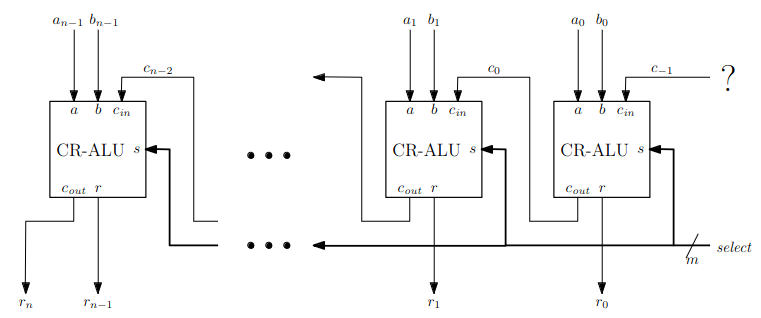
\includegraphics[width=300pt]{figures/CR-ALU.png}
\end{exercisenoinc}

\begin{requirementsnoinc}
    \center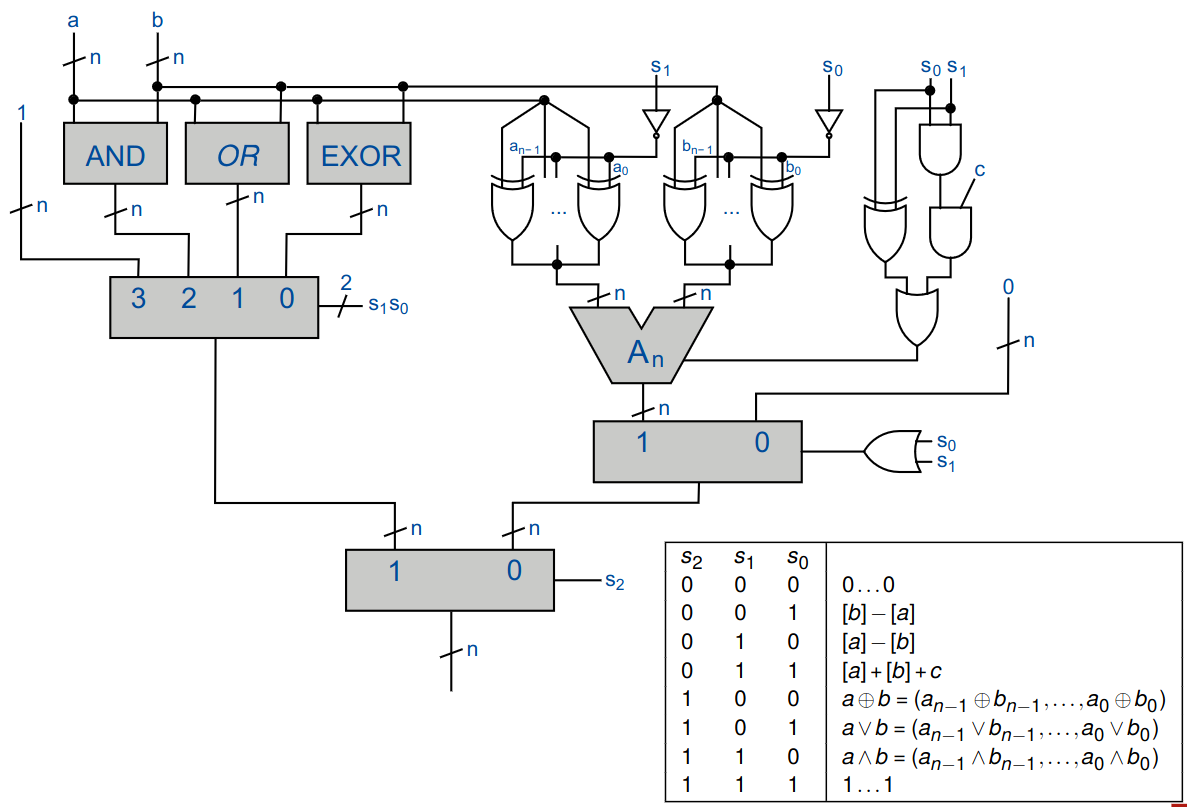
\includegraphics[width=240pt]{figures/ALU_logic.png}
\end{requirementsnoinc}

\begin{solutionnoinc}
    \center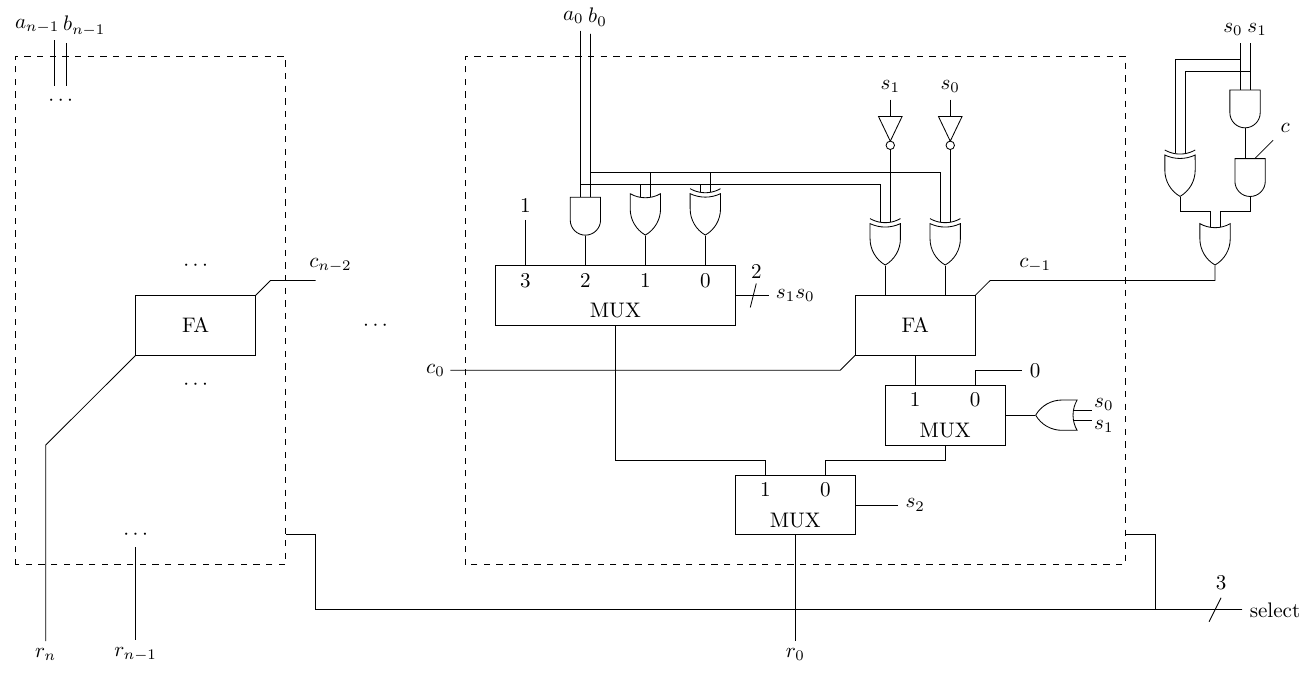
\includegraphics[width=240pt]{figures/CR-ALU-Cell.png}
\end{solutionnoinc}

\begin{solutionnoinc}
CR-ALU ist wie auf vorheriger Folie bei $n=1$ mit folgenden Änderungen:
    \begin{itemize}
        \item $A_n$ ist ein Volladdierer
        \item Es gibt einen weiteren Ausgang an $A_n$, um das Carry für die nächste Zelle zu übergeben
        \item $c$ wird direkt in den Volladdierer übergeben
        \item Die wegfallende Schaltung erzeugt $c_{-1}$
    \end{itemize}
\end{solutionnoinc}

\end{frame}
